\chapter{Introduction to Vehicular Communications}
\section{Principles and challenges}

L'obiettivo principale è quello dell'\textbf{Intelligent Transportation System} (ITS), ovvero un sistema che permetta di migliorare la sicurezza, la mobilità e l'efficienza del trasporto che sono composti di hardware, software e communication technologies.

Alcuni esempi di ITS sono:
\begin{itemize}
  \item \textbf{Infotainment Sustainability}
  \item \textbf{Tolling}
  \item \textbf{Emergency Call}
  \item \textbf{Crash Imminent Safety}
\end{itemize}

Solitamente le ITS Applications sono isolate e non permettono il passaggio di dati da una app all'altra, mentre le C-ITS(Cooporative ITS) sono applicazioni che permettono la cooperazione tra veicoli e infrastrutture.

Tutte le informazioni raccolte dai sensori del veicolo vengono raccolti e inviati alle \textbf{Engine Control Units(ECUs)} che sono sistemi integrati che controllano ona o più funzioni del veicolo.


Si utilizzano i sistemi BUS per effettuare il passaggio di informazioni fra le ECUs(che ora si chiamano Electronic Control Units) e i sensori del veicolo.

Applicazioni visionarie basate sulla comunicazione fra veicoli:
\begin{itemize}
  \item Lane assistant
  \item Lateral collision
  \item Accident reporting
  \item Intersection assistace
  \item cooperative driving
\end{itemize}



Le principali difficoltà della comunicazione sono:
\begin{itemize}
  \item \textbf{Basic}
  \begin{itemize}
    \item latenza
    \item throughput
  \end{itemize}
  \item \textbf{Communication in veichles}
  \begin{itemize}
    \item robustezza
    \item costo
  \end{itemize}
  \item \textbf{Communication between veichles}
  \begin{itemize}
    \item privacy
    \item sicurezza
    \item reachability
    \item interoperabilità
  \end{itemize}
\end{itemize}





\section{Standardization and open issues}

Il gruppo di lavoro \textbf{ISO/TC 204} per le standardizzazioni è responsabile per la maggiorparte degli aspetti architetturali per gli ITS, ha prodotto il concetto \textbf{Communications Access for Land Mobiles(CALM)} e \textbf{ETSI TC ITS} basato sui recenti C-ITS europei.



\subsection{CALM}
Soluzione a strati che permette comunicazioni:
\begin{itemize}
  \item \textbf{V2V}: Veichle to Veichle
  \item \textbf{V2I}: Veichle to Infrastructure
  \item \textbf{I2I}: Infrastructure to Infrastructure
\end{itemize}

Sfrutta la comunicazione multichannel, capace di connettersi a tanti gestori e utilizza IPv6. 

Tecnologia che è in grado di selezionare il mezzo di comunicazioni migliroe per l'occasione.

\begin{figure}[!ht]
  \centering
  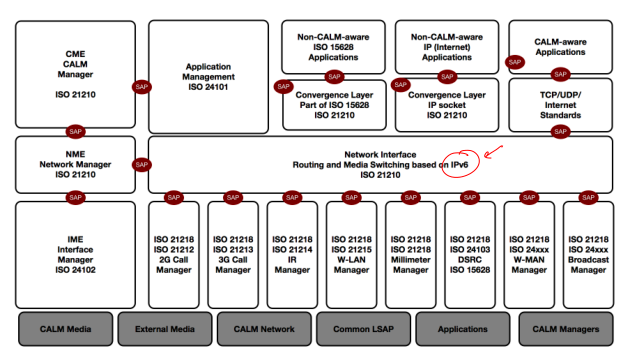
\includegraphics[width=0.4\textwidth]{./images/CALM.png}
  \caption{CALM architecture}
  \label{fig:CALM}
\end{figure}


\subsection{Visione Europea}
L'Europa è leader mondiale in ITS(probabilmente per industria dell'automotive) ed è conscia delle quantità di denaro, energia e impatto di CO2 causate dalle congestioni stradali.

L'obiettivo europeo è quello di raggiungere \textbf{zero incidenti, zero ritardi, meno impatto sull'ambiente, persone informat, servizi accessibili, rispetto della privacy e sicurezza.}

Lo sviluppo è portato avanti dalle aziende del territorio.

\subsection{Visione Americana}
In america lo sviluppo è mandato avanti da fondi statali, vengono elargiti programmi di 5 anni per lo sviluppo di ITS.

L'approccio americano porta all'utilizzo sia di tecnologie \textbf{non-DSRC(Dedicated Short Range Communications)} che di tecnologie \textbf{DSRC} per l'utilizzo rispettiamente di segnali a lunga distanza come la rete cellulare oppure di segnali a corto raggio come le onde radio.




\section{ITS Architecture}

Data la granded quantità di persone nel mondo pronte a sviluppare ITS, si è introdotto il concetto di \textbf{ITS-S(ITS station)} che rappresenta un \textbf{set di istruzioni} per lo sviluppo di un ITS.

Da un punto di vista architetturale il ITS-S è simile al modello OSI, nasce cosi l'architettura \textbf{ITSC} che ruota attorno alle ITS station, una unità computazionale modulare.

Questo porta alla realizzazione di diversi ITS:
\begin{itemize}
  \item Vehicle ITS
  \item Roadside ITS
  \item Central ITS
  \item Personal ITS
\end{itemize}


\begin{figure}[!ht]
  \centering
  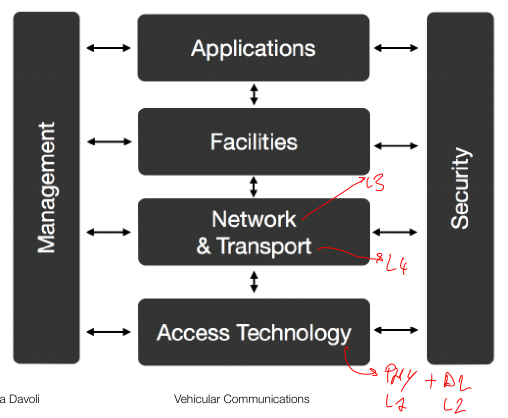
\includegraphics[width=0.4\textwidth]{./images/its_architecture.png}
  \caption{ITS architecture}
  \label{fig:its_architecture}
\end{figure}


L'host ITS-S è composto da:
\begin{itemize}
  \item 4 layer logici orizzonatali
  \begin{itemize}
    \item \textbf{Access technologies} layer: unisce layer fisico e layer data link del sistema ISO/OSI
    \item \textbf{Networking e transport} layer: corrisponde ai layer Networking e layer Transport del sistema ISO/OSI 
    \item \textbf{Facilities layer}: corrisponde al layer Session, Presentation e Application del sistema ISO/OSI
    \item \textbf{Application} layer: composto dalle applicazioni ITS-s e costruito sui precedenti tre layer
  \end{itemize}
  \item 2 layer verticali
\end{itemize}


L'\textbf{architettura wave} è un sotto gruppo di funzionalità proposte dall'architettura \autoref{fig:its_architecture} e omette l'implementazione per lo strato \textbf{Facilities} e \textbf{Application}.

\begin{figure}[!ht]
  \centering
  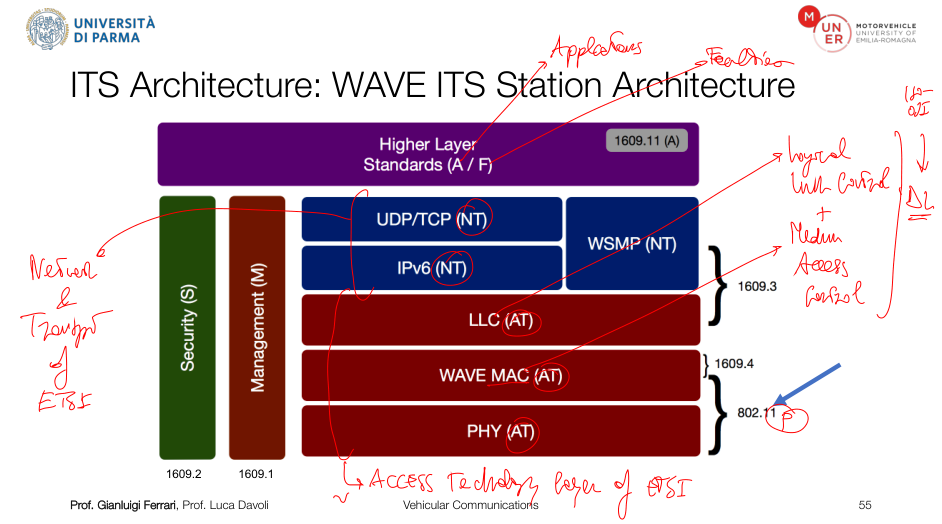
\includegraphics[width=0.8\textwidth]{./images/wave_architecture.png}
  \caption{WAVE architecture}
  \label{fig:wave_architecture}
\end{figure}


La comunicazzione nell'architettura di tipo WAVE è categorizzabile in due:
\begin{itemize}
  \item data-plane: per funzioni data driven come infotainment
  \item management-plane: per funzioni come la frenata, ecc
\end{itemize}

WAVE ha un suo protocollo per la comunicazione che prende il nome di \textbf{WSMP(WAVE Short Message Protocol)} e serve per effettuare le comunicazioni tra veicoli in movimento.


\subsection{Applicazioni ITS}

\begin{figure}[!ht]
  \centering
  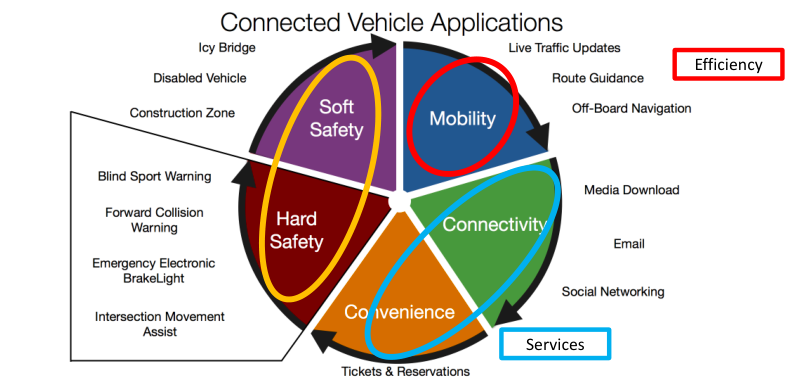
\includegraphics[width=0.8\textwidth]{./images/its_apps.png}
  \caption{ITS applications}
  \label{fig:its_apps}
\end{figure}


\section{Autonomous driving}
\subsection{NHSTA Levels - USA}
\begin{itemize}
  \item \textbf{Level 0}: no automation
  \item \textbf{Level 1}: Funzioni individuali sono automatizzate(frenata, stabilità ecc)
  \item \textbf{Level 2}: Almeno 2 o più controlli sono automatizzati e comunicano fra di loro(adaptive cruise control, lane keep assist)
  \item \textbf{Level 3}: Il veicolo è in grado di gestire tutte le funzioni di guida in determinate condizioni
  \item \textbf{Level 4}: Il veicolo è in grado di gestire tutte le funzioni di guida e l'umano non deve prende mai il controllo
\end{itemize}


\subsection{SAE Levels - Europe}

\begin{itemize}
  \item \textbf{Level 0}: no automation
  \item \textbf{Level 1}: hands on(adaptive cruise control, parking assistances)
  \item \textbf{Level 2}: hands off(il sistema prende controllo totale e se non riesce a gestire la situazione da il controllo all'umano)
      \item \textbf{Level 3}: eyes off(guidatore presente al posto di guida per necessita di emergenze ma può fare altro come leggere ecc)
      \item \textbf{Level 4}: mind off(umano non deve fare niente)
      \item \textbf{Level 5}: no driver(no volante)
\end{itemize}
